\documentclass[12pt]{beamer}
\usetheme{Madrid}
\usecolortheme{default}

\usepackage{ragged2e}
\usepackage[utf8]{inputenc}
\usepackage[brazil]{babel}
\usepackage[T1]{fontenc}
\usepackage{xcolor}
\usepackage{amsmath}
\usepackage{amsfonts}
\usepackage{amssymb}
\usepackage{graphicx}
\usepackage{setspace}
\setbeamertemplate{caption}[numbered]
\usepackage{hyperref}



\addtobeamertemplate{block begin}{}{\justifying}
\addtobeamertemplate{block alerted begin}{}{\justifying}
\addtobeamertemplate{block example begin}{}{\justifying}
\let\raggedright\justifying         
\AtBeginEnvironment{frame}{\justifying} 

\newcounter{questao} 

\newcommand{\novaquestao}[2][]{%
	\stepcounter{questao}%
	\begin{frame}{Questão \thequestao\ifx&#1&\else\ -- #1\fi}%
		\justifying
		#2
	\end{frame}%
}


\author[Joao Victor]{% 
	Joao Victor\inst{1}}
\title{Revisão - Análise Combinatória}
\institute[]{% 
	\textsuperscript{1} Instituto Federal do Amazonas (IFAM) \\
}
\date{\today} 
%\titlegraphic{
\includegraphics[width=0.3\textwidth]{imagens/logo.png}}

%\subject{}

% ---------------------------------------------------------

\begin{document}
	\onehalfspacing 
	
	\begin{frame}
		\titlepage
	\end{frame}
	
	\section{Aplicações}
	
	\novaquestao{
		Lançando simultaneamente um dado e uma moeda, quantos são os possíveis resultados?
	}
	
	\novaquestao{
		Uma montadora de automóveis apresenta um carro em quatro modelos diferentes e em cinco cores diferentes. Um consumidor que quiser adquirir esse veículo terá quantas opções de escolha? %20
	}
	
	\novaquestao{
		Quantos números naturais de três algarismos podem ser formados com os algarismos 1, 2, 6, 8 e 9? %125
	}
	
	\novaquestao{
		Quantos números naturais de três algarismos distintos podem ser formados com os algarismos 1, 2, 6, 8 e 9? 
		%60
	}
	
	\begin{frame}
		\begin{alertblock}{Princípio Fundamental da Contagem}
			Se um experimento A apresenta $n$ resultados distintos e um experimento B apresenta K resultados distintos, então o experimento composto de A e B, nessa ordem, apresenta $nk$ resultados distintos.
		\end{alertblock}
	\end{frame}
	
	\novaquestao{
		Quantos números naturais de três algarismos distintos podem ser formados com os algarismos 0, 1, 2, 6 e 8?
		
		%48
	}
	
	\novaquestao{
		Quantos divisores naturais possui o número 72? %12
	}
	
	\section{Principio Aditivo de contagem}
	
	\novaquestao{
		Durante um exame médico, foram medidas as estaturas dos alunos de uma classe. Observou-se que dezenove alunos têm estatura até $1,70\ m$ e dez alunos têm estatura maior do que $1,70\ m$. Quantos alunos havia na classe? %29
	}
	
	\novaquestao{
		O professor de português pediu para que os alunos de uma classe lessem pelo menos uma das obras, \textit{Dom Casmurro} ou \textit{O alienista}, de Machado de Assis. Após algum tempo, o professor constatou que:
		
		\begin{itemize}
			\item cada aluno havia lido pelo menos uma das obras;
			\item 22 alunos havia leram \textit{Dom Casmurro}
			\item dezoito alunos, \textit{O Alienista}
			\item dez alunos, as duas obras
		\end{itemize} Quantos alunos há na classe? %30
	}
	
	\novaquestao{
		Quantos números naturais de quatro ou cinco algarismos distintos podem ser formados com os algarimos 1, 2, 3, 4, 5 e 6? %1080
	}
	
	\novaquestao{
		Com os algarismos 1, 2, 3, 4, 5 e 6, quantos números naturais de quatro algarismos distintos podem ser formados de modo que o algarismo das unidades seja par ou o algarismo dos milhares seja ímpar? %252
	}
	
	\begin{frame}
		\begin{alertblock}{Princípio aditivo de contagem}
			Sendo A e B conjuntos finitos, o número de elementos da união de A e B é dado por $n(A \cup B) = n(A)+n(B)-n(A \cap B)$, onde o símbolo $n()$ representa o número de elementos do conjunto indicado entre parênteses.
		\end{alertblock}
	\end{frame}
	
	\novaquestao{
		Quais dos seguintes agrupamentos são \textbf{arranjos} simples? Por quê?
		
		\begin{itemize}
			\item Com os algarismos 1, 2, 3 e 4, formam-se agrupamentos, sendo que cada agrupamento representa um número natural de três algarismos distintos.
			
			\item Com os pontos A, B, C e D da circunferência ao abaixo, formam-se agrupamentos, sendo que casa agrupamento representa os vértices de um triângulo.
			
			\begin{center}
				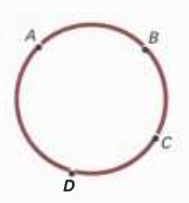
\includegraphics[scale=0.4]{imagem/arranjo}
			\end{center}
		\end{itemize}
	}
		
	\begin{frame}
		\begin{alertblock}{Arranjo simples}
			Seja $I=\left\lbrace a_1,a_2,a_3,...,a_n\right\rbrace $ um conjunto formado por n elementos e seja p um número natural não-nulo tal que $p \leq n$. Chama-se "\textbf{arranjo simples} de p elementos de $I$" toda sequência formada por p elementos de $I$ distintos.
		\end{alertblock}
	\end{frame}
	
	\novaquestao{
		Os arranjos simples dos elementos do conjunto $I=\left\lbrace 5, 6, 7, 8\right\rbrace$ tomados dois a dois são?
	}
	
	\novaquestao{
		Calcular $A_{6,4}$
	}
	
	\novaquestao{
		jslaskkasl
	}
\end{document}